\documentclass[11pt]{article}
\usepackage[margin=1in]{geometry}
\usepackage{graphicx}
\usepackage{amsmath}
\usepackage{verbatim}
\graphicspath{{../../Screenshots/}}
\begin{document}
\section{MC Uncertainty Propagation}
For a data reduction equation (DRE) of the form:
$$r = f(x_1, x_2, \dots, x_L)$$
\begin{itemize}
    \item Generate random values for each of the inputs
    \item For each set of random values, evaluate random
    \item This generates a set of values r=\{$r_1, r_2, \dots , r_m$\}
    \item Then evaluate the statistics of the set r
\end{itemize}
\begin{center}
    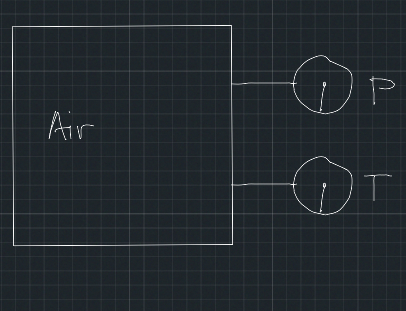
\includegraphics[width = 200pt]{Screenshot 2025-12-03 135441.png}
\end{center}
After you perform uncertainty analyses on the measured T and P value, calculate an uncertainty interval for density $$\rho = \frac{P}{R_{air}T}$$
\section{MC analysis}
\begin{align*}
    r &= \rho
    \\x_1 &= p
    \\x_2 &= T
   \\ x_3 &= R_{air}
\end{align*}
Suppose:
\\
$\bar{T}=298$, $U_t=2k$\\
$T = 298\pm 2k (95\%)$\\
$P = \bar{P}\pm U_pk (95\%)$\\
$P = 100\pm 1k (95\%)$

\newpage
\subsection{the code for this is:}
\begin{verbatim}
m<-2e5 # of MC replicates

P <- numeric(M)

t <- numeric(M)

rho <- numeric(M)

Rair <- 287

for (m in 1:M) {
    p[m] <- rnorm(n=1, mean=1e5, sd = 500)
    t[m] <- rnorm(n=1, mean=298, sd = 1)
    rho[m] <- p[m]/Rair/t[m]
}
P<-0.95#conf.level
Pmin <- (1-p)/2
Pmax<-(1+p)/2
quantile(rho,probs=c(Pmin,Pmax))
\end{verbatim}
The quantile function works on a list of numbers
$\rho={\rho_1, ..., \rho_M}$ sorted from smallest to largest 
\\
For P = 95\%, the quantile function finds the $\rho$ values that correspond to the upper and lower limits of 95\% of the values.
\begin{verbatim}
x = {1,2,3, .. ,100}
quantile(x,probs = c(Pmin,Pmax)) 

Pmin=(1-p)/2 = 0.025
Pmax=(1+p)/2=0.975
\end{verbatim}
\section{Manufacturer's correlation}
$$\dot{m}=c(\rho_oZ)^{1/2}$$
$$r=x_1(x_2x_3)^{1/2}$$
\begin{tabular}{|c|c|c|c|}
    \hline
    Units & Quantity & Mean Value & $u = (s^2+b^2)^{1/2}$
    \\\hline
    ?&c&0.0504&0.0000005
    \\\hline
    $kg/m^2$&$\rho_P$&1.15&0.2
    \\\hline
    -&-&-&-
\end{tabular}
\\~\\
\begin{center}
    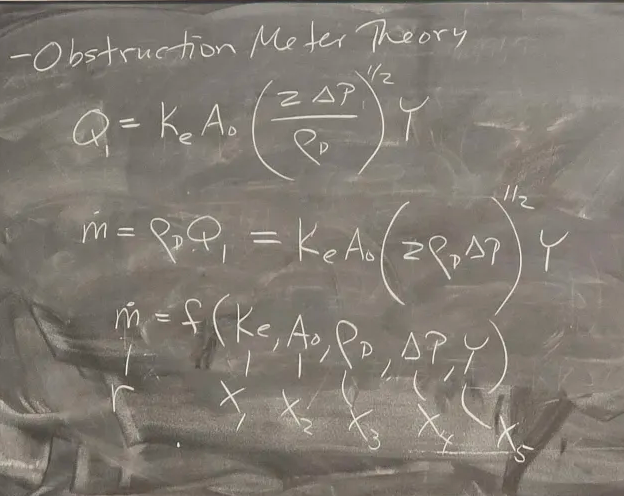
\includegraphics[width = 200pt]{Screenshot 2025-12-03 140130.png}
\end{center}
\section{Numerical Integration}
$$\dot{m}=2\pi\int_{0}^{R}\rho rvdr$$
$$\dot{m}=2\pi\rho\int_{0}^{R}rvdr$$
Where: $v=\big(\frac{2\Delta P}{\rho_0}\big)^{1/2}$ Bernoulli Eqn.
\\
$$\dot{m}=2\pi\rho\int_{0}^{R}r\big(\frac{2\Delta P}{\rho_0}\big)^{1/2}dr$$
$$\dot{m}=2\pi\rho\big(\frac{2}{\rho_0}\big)^{1/2}\int_{0}^{R}r\Delta P^{1/2}dr$$
\begin{center}
    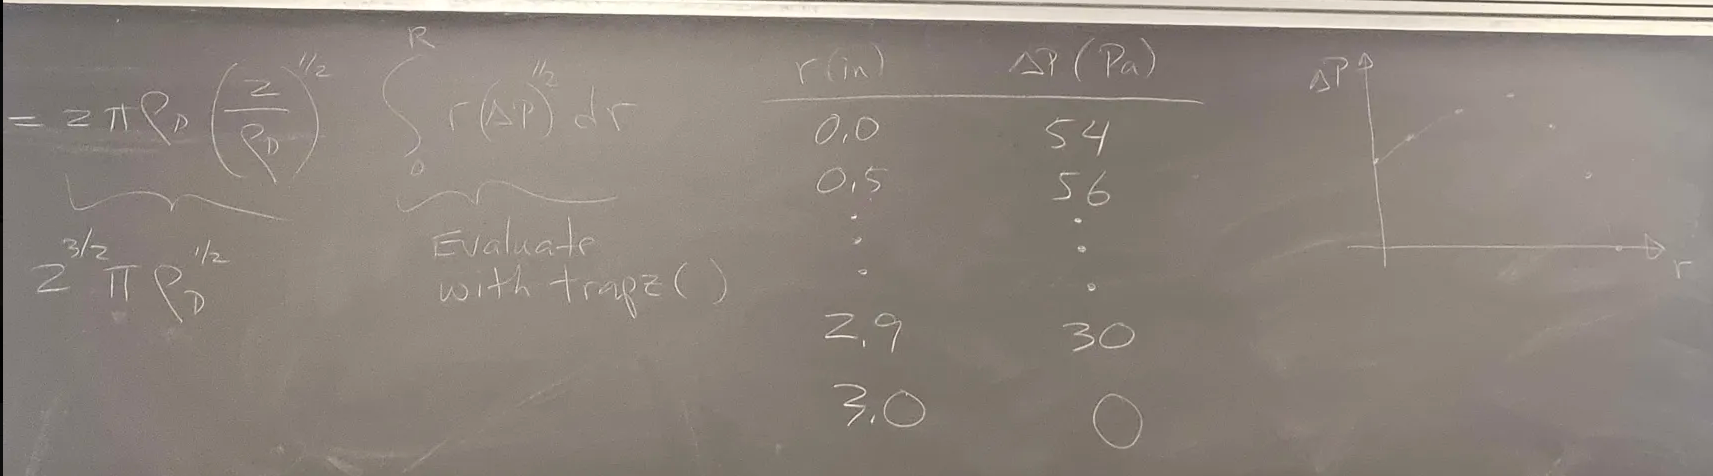
\includegraphics[width=\textwidth]{Screenshot 2025-12-03 140632.png}
\end{center}
\subsubsection{algorithm}
\begin{itemize}
    \item generate a random value for $\rho_o$:
    \\rhoD $<-$ rnorm(n=1,mean=$\bar{\rho}_0$, sd = $u_{\rho_0}$)
    
    \item Generate one random value for each of the r values
    \begin{verbatim}
    r1<-rnomr(n=1,mean=rbar1, sd = ur1)
    r2<-rnomr(n=1,mean=rbar2, sd = ur2)
    \end{verbatim}
    \item Generate one random value for each of the $\Delta P$s
    \\
    dP1$<$-rnorm(n=1, mean = 54, sd = $U_{\Delta P_1})$
    
\end{itemize}
\begin{center}
    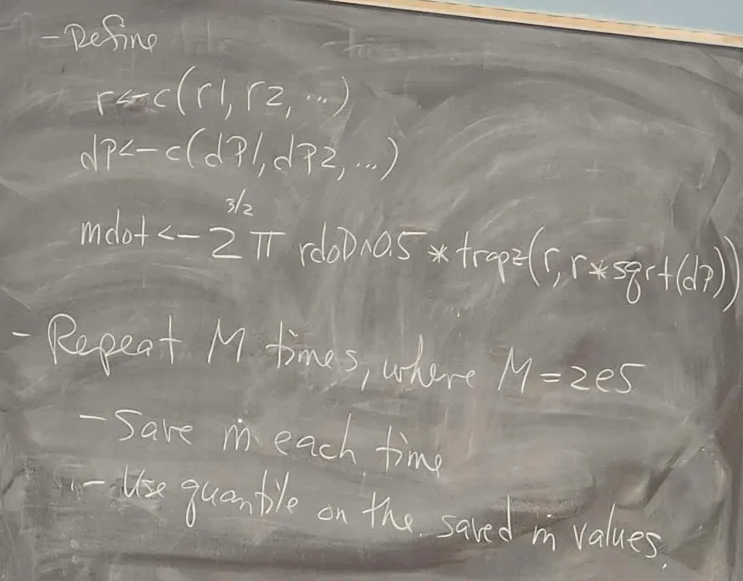
\includegraphics[width=250pt]{Screenshot 2025-12-03 140911.png}
\end{center}
educational
YWMzZGE2OTAzNjk4NTY4ZTQxZTgzNWEx
\end{document}